\section{Event Selection and Object Definitions}
\label{sec:hh_event_selection}

%%%%%%%%%%%%%%%%%%%%%%%%%%%%%%%%%%%%%%%%%%%%%%%%%%%%%%%%%%%%%%%%%%%%%%%%%%%%%%
%%%%%%%%%%%%%%%%%%%%%%%%%%%%%%%%%%%%%%%%%%%%%%%%%%%%%%%%%%%%%%%%%%%%%%%%%%%%%%
%%%%%%%%%%%%%%%%%%%%%%%%%%%%%%%%%%%%%%%%%%%%%%%%%%%%%%%%%%%%%%%%%%%%%%%%%%%%%%
%
% TRIGGER STRATEGY
%
%%%%%%%%%%%%%%%%%%%%%%%%%%%%%%%%%%%%%%%%%%%%%%%%%%%%%%%%%%%%%%%%%%%%%%%%%%%%%%
%%%%%%%%%%%%%%%%%%%%%%%%%%%%%%%%%%%%%%%%%%%%%%%%%%%%%%%%%%%%%%%%%%%%%%%%%%%%%%
%%%%%%%%%%%%%%%%%%%%%%%%%%%%%%%%%%%%%%%%%%%%%%%%%%%%%%%%%%%%%%%%%%%%%%%%%%%%%%
\subsection{Trigger Strategy}
\label{sec:hh_trigger_strategy}

The $h \rightarrow WW^*$ decay, from which the leptons in the final state arise,
is characterized by a sub-leading lepton which has typically quite low \pT~as a result
of one of the $W$-bosons being off-shell.
If the analysis is to record the dilepton $hh \rightarrow \bbww$ events, then, it is important
to minimize the \pT~thresholds on at least one of the leptons in the event so that the
signal events do not get discarded at the level of the trigger.
As a result, the trigger strategy used in the dilepton $hh \rightarrow \bbww$ analysis is based
on a combination of single and dilepton triggers.
The single lepton triggers typically enforce higher \pT~thresholds on the single leading lepton
than those encountered in the dilepton triggers, but they do not make any requirement on the sub-leading
lepton candidate.
Events with sub-leading leptons below the dilepton triggers' thresholds, then, have a chance of
being recorded and kept for use in the analysis.

The typical \pT~thresholds for the single-lepton triggers used in the present analysis are $26-28$\,GeV.
There are two types of dilepton triggers used in the analysis: `symmetric' and `asymmetric'.
Symmetric triggers enforce trigger \pT~thresholds that are roughly the same for both the leading and subleading
online lepton, and are typically around $20\,\GeV$.
The asymmetric triggers require relatively low \pT~thresholds (lower than single lepton \pT~thresholds)
on the leading lepton, but very low thresholds (typically around 7\,GeV) on the sub-leading lepton.
The asymmetric triggers are only defined for dilepton events where the leptons have different-flavor ($e \mu$ or $\mu e$ events).

The trigger strategy is illustrated in Figure~\ref{fig:hh_trig_flowchart}.
The single lepton triggers are given priority as they make no kinematic requirements on the
sub-leading leptons in the event.
Both leptons in the event are checked for having fired corresponding single lepton trigger before
checking the dilepton triggers.
If the event has a different-flavor lepton pair, the asymmetric triggers are given priority over the symmetric ones due to their having
lower \pT~thresholds on the sub-leading lepton.
The trigger strategy outlined in Figure~\ref{fig:hh_trig_flowchart} is $\sim 95\%$ efficient for events
with leading (subleading) lepton \pT~values of 28\,GeV (20\,\GeV) and $\sim 90\%$ efficient for events
with subleading leptons having \pT~values below 20\,GeV.

\begin{figure}[!htb]
    \begin{center}
        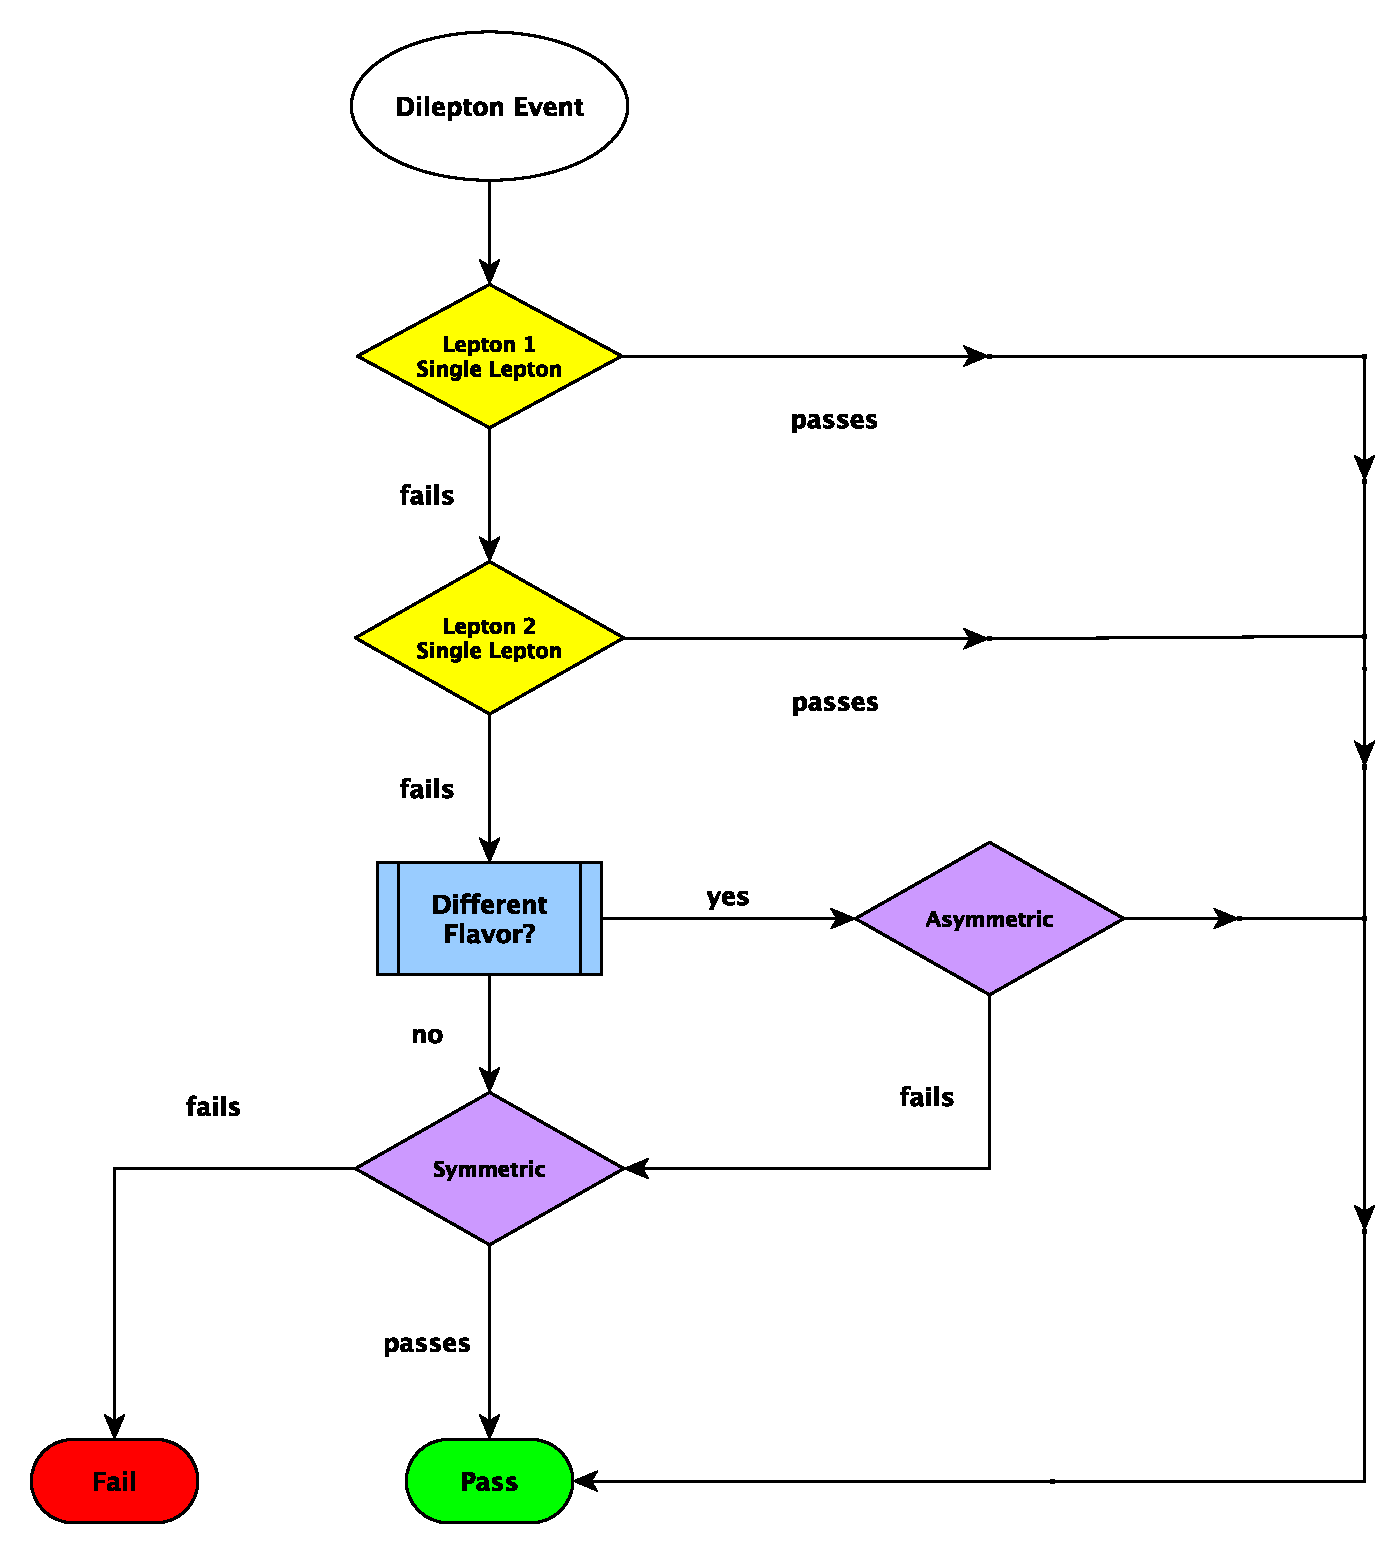
\includegraphics[width=0.65\textwidth]{figures/common_ana/trig/updated_trigger_logic_feb26PDF}
        \caption{
            Flowchart illustrating the implementation of the trigger strategy used in the
            search for the dileptonic $hh \rightarrow \bbww$.
            The diamonds indicate points at which a specific trigger is checked.
            The yellow diamonds refer to the single lepton triggers associated with one of the leptons in the event.
            The purple diamonds refer to testing of dilepton triggers.
            In the figure, `Asymmetric' and `symmetric' refers to the asymmetric and symmetric different-flavor
            dilepton triggers, respectively.
            The red `Fail' and green `Pass' terminations refer to the event failing and succeeding,
            respectively, the trigger logic.
            Only events that pass are kept and considered in the analysis.
        }
        \label{fig:hh_trig_flowchart}
    \end{center}
\end{figure}

%%%%%%%%%%%%%%%%%%%%%%%%%%%%%%%%%%%%%%%%%%%%%%%%%%%%%%%%%%%%%%%%%%%%%%%%%%%%%%
%%%%%%%%%%%%%%%%%%%%%%%%%%%%%%%%%%%%%%%%%%%%%%%%%%%%%%%%%%%%%%%%%%%%%%%%%%%%%%
%%%%%%%%%%%%%%%%%%%%%%%%%%%%%%%%%%%%%%%%%%%%%%%%%%%%%%%%%%%%%%%%%%%%%%%%%%%%%%
%
% OBJECT DEFINITIONS
%
%%%%%%%%%%%%%%%%%%%%%%%%%%%%%%%%%%%%%%%%%%%%%%%%%%%%%%%%%%%%%%%%%%%%%%%%%%%%%%
%%%%%%%%%%%%%%%%%%%%%%%%%%%%%%%%%%%%%%%%%%%%%%%%%%%%%%%%%%%%%%%%%%%%%%%%%%%%%%
%%%%%%%%%%%%%%%%%%%%%%%%%%%%%%%%%%%%%%%%%%%%%%%%%%%%%%%%%%%%%%%%%%%%%%%%%%%%%%
\subsection{Object Definitions}
\label{sec:hh_object_def}

This section describes the definitions and working points of the leptons and jets used
in the search for dilepton $hh \rightarrow \bbww$.
The lepton definitions are given in Table~\ref{tab:hh_lepton_def} and the jet definitions are
given in Table~\ref{tab:hh_jet_def}.
Discussion of the working points for lepton identification and isolation is given in
Section~\ref{sec:leptons}.
That of jets is found in Section~\ref{sec:jets} and \ref{sec:flavor_tagging}, for
jets, generically, and $b$-tagged jets, respectively.

The \pT~requirements of the leptons depends on the trigger used to select the event.
That is, the point in the flowchart in Figure~\ref{fig:hh_trig_flowchart} at which
a trigger fires defines the offline \pT~threshold applied to the lepton: it is taken
to be 2\,GeV above the threshold of the fired trigger.
Given the use of a wide set of single lepton and dilepton triggers, this threshold
can vary between 19-28\,GeV for the leading leptons and 10-17\,GeV for the sub-leading leptons.
As in the analysis discussed in Chapter~\ref{chap:search_stop},
the lepton isolation requirements are rather loose, given that a large contamination of
fake and non-prompt leptons is not expected as a result of the requirement of two relatively
high-\pT~leptons.
The requirements on the impact parameter quantities $|d_0 / \sigma_{d_0}|$ and $|z_0 \times \sin \theta|$
further ensure that the leptons are likely to be prompt and have originated
from the primary hard-scatter vertex.

\begin{table}[!htb]
    \begin{center}
    \caption{
        Lepton definitions for the analysis searching for dilepton $hh \rightarrow \bbww$.
    }
    \label{tab:hh_lepton_def}
        \begin{tabular}{l | c | c | c | c }
        \hline
        \hline
            & \multicolumn{4}{c}{\textbf{Leptons}} \\
        \cline{2-5}
            & \multicolumn{2}{c}{\textbf{Electrons}} & \multicolumn{2}{c}{\textbf{Muons}} \\
        \cline{2-5}
            & \textbf{Baseline} & \textbf{Signal} & \textbf{Baseline} & \textbf{Signal} \\
        \hline
        \pT~requirement [GeV] & $(>10,>10)$ & $\begin{matrix} \text{Trig. threshold} \\ \text{+2 GeV} \end{matrix} $ & $(>10,>10)$ & $\begin{matrix} \text{Trig. threshold} \\ \text{+2 GeV} \end{matrix} $ \\
        $|\eta|$ requirement & \multicolumn{2}{c}{$<2.47$} & \multicolumn{2}{c}{$<2.4$} \\
        Identification WP & \texttt{Loose} & \texttt{Tight} & \multicolumn{2}{c}{\texttt{Medium}} \\
        Isolation & \multicolumn{4}{c}{\texttt{GradientLoose}} \\
        $|d_0 / \sigma_{d_0}|$ & $--$ & $<5$ & $--$ & $<3$ \\
        $|z_0 \times \sin \theta|$ [mm] & $--$ & $<0.5$ & $--$ & $<0.5$ \\
        \hline
        \hline
        \end{tabular}
    \end{center}
\end{table}

\begin{table}[!htb]
    \begin{center}
    \caption{
        Jet definitions for the analysis searching for dilepton $hh \rightarrow \bbww$.
    }
    \label{tab:hh_jet_def}
        \begin{tabular}{l | c | c}
            \hline
            \hline
                & \textbf{Jets} & \textbf{$b$-tagged Jets} \\
            \hline
            \pT~requirement [GeV] & \multicolumn{2}{c}{$>20$} \\
            $|\eta|$ requirement & $<2.8$ & $<2.4$ \\
            Pileup suppression & \multicolumn{2}{c}{ $\texttt{JVT} > 0.59$ if $\pT<60\,\GeV$~ and $|\eta| < 2.4$} \\
            Flavor-tagging WP & $--$ & $70\%$ \\
            \hline
            \hline
        \end{tabular}
    \end{center}
\end{table}



%%%%%%%%%%%%%%%%%%%%%%%%%%%%%%%%%%%%%%%%%%%%%%%%%%%%%%%%%%%%%%%%%%%%%%%%%%%%%%
%%%%%%%%%%%%%%%%%%%%%%%%%%%%%%%%%%%%%%%%%%%%%%%%%%%%%%%%%%%%%%%%%%%%%%%%%%%%%%
%%%%%%%%%%%%%%%%%%%%%%%%%%%%%%%%%%%%%%%%%%%%%%%%%%%%%%%%%%%%%%%%%%%%%%%%%%%%%%
%
% BJET MOMENTUM CORRECTIONS
%
%%%%%%%%%%%%%%%%%%%%%%%%%%%%%%%%%%%%%%%%%%%%%%%%%%%%%%%%%%%%%%%%%%%%%%%%%%%%%%
%%%%%%%%%%%%%%%%%%%%%%%%%%%%%%%%%%%%%%%%%%%%%%%%%%%%%%%%%%%%%%%%%%%%%%%%%%%%%%
%%%%%%%%%%%%%%%%%%%%%%%%%%%%%%%%%%%%%%%%%%%%%%%%%%%%%%%%%%%%%%%%%%%%%%%%%%%%%%
\subsection{Corrections to the $b$-tagged Jet Momenta}
\label{sec:hh_bjet_correction}

In the search for dileptonic $hh \rightarrow \bbww$, we apply the so-called `muon-in-jet' energy
correction to all $b$-tagged jets.
This correction is used to correct the four-vector of all $b$-tagged jets on a \textit{per-jet} basis
by attempting to recover unaccounted for energy and momentum due to semileptonic $b$-decays within the
$b$-tagged jets.
As illustrated in Figure~\ref{fig:bjet_semileptonic}, in $b$-quark decays occuring in the $b$-tagged jets
where you have at least a single decaying $W$-boson, you will have the possibility of having at least one lepton
contained within the $b$-tagged jet.
The $W$-boson decays at essentially equal rates to all flavors of leptons, however we cannot efficiently
the electrons and hadronic $\tau$ decays occuring inside of jets.
We can, however, identify muons originating from in-flight decays within jets, as they do not deposit
a significant amount of energy within the jet and escape the calorimeter.
The electron and $\tau$ energy deposits, on the other hand, will for the most part be contained within
the jet and so their energy is, at least partially, accounted for in the jet reconstruction.

As the escaping muon's energy and momenta are not fully taken into account when reconstructing the $b$-tagged jets,
it is important to see if we can recover this lost energy.
The aim being to improve the $b$-tagged jet energy response and therefore improve the resolution of the invariant
mass of the reconstructed $bb$-system, $m_{bb}$, which peaks at $m_{h} = 125\,\GeV$ in the $hh$ signal
being searched for.
As will be seen in Section~\ref{sec:hh_strategy}, the current analysis requires that signal events
have $m_{bb}$ within a small window about $m_{h}$.
If we can improve the $m_{bb}$ resolution, then we can increase the signal purity of this selection.

The muon-in-jet correction proceeds as follows.
Any muons satisfying the baseline requirements described in Table~\ref{tab:hh_lepton_def} that
are also with $\Delta R = 0.4$ of a $b$-tagged jet are first identified.
The \textit{nearby} muon with the highest \pT~ then has its four-momentum `added back' to the reconstructed
$b$-tagged jet.
Muons deposit, on average, $3-4\,\GeV$ of energy in the calorimeter.
Once a muon's four momentum has been added back to the $b$-tagged jet in question, the calorimeter
energy deposit of the muon is subtracted away from the $b$-tagged jet's four momenta so as to avoid double
counting of the calorimeter energy: once from the muon, now considered part of the $b$-tagged jet, and a
second time from the energy deposit already having been used in the jet reconstruction.

Figure~\ref{fig:bjet_correction} shows the $m_{bb}$ distribution for the dilepton
$hh \rightarrow \bbww$ signal process before and after performing the muon-in-jet correction
as described above.
With the $m_{bb}$ selections described in Section~\ref{sec:hh_strategy}, the muon-in-jet
correction increases the $hh$ signal acceptance by roughly $5-7\%$ (depending on any additional
selections being applied on top of the $m_{bb}$ ones).

\begin{figure}[!htb]
    \begin{center}
        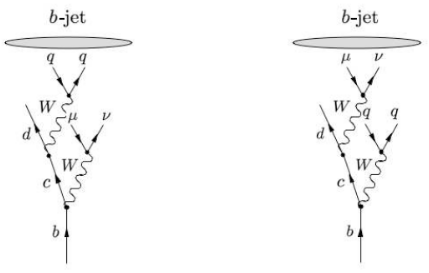
\includegraphics[width=0.45\textwidth]{figures/search_hh/bjet_semileptonic}
        \caption{
            Diagrams illustrating the semileptonic weak decays of the $b$- and $c$-quarks initiating the reconstruction
                of a $b$-tagged jet.
                The muons and neutrinos escape the calorimeter and their momenta and energy are not accounted
                for in the $b$-tagged jet reconstruction.
        }
        \label{fig:bjet_semileptonic}
    \end{center}
\end{figure}

\begin{figure}[!htb]
    \begin{center}
        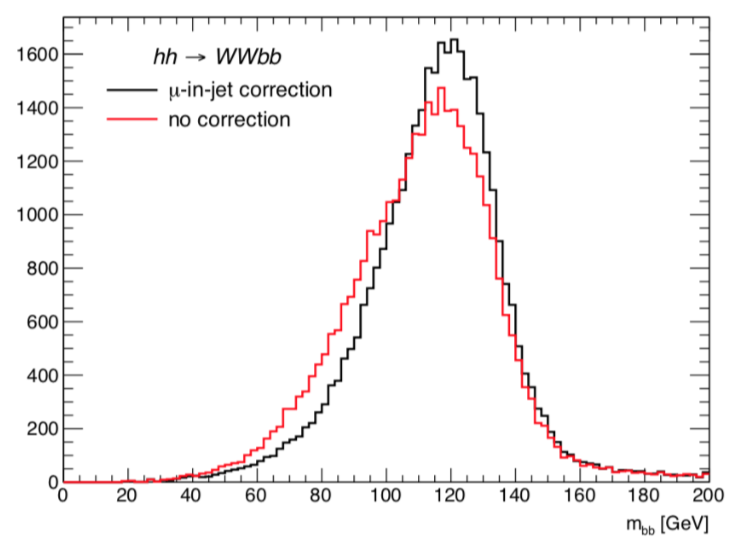
\includegraphics[width=0.6\textwidth]{figures/search_hh/bjet_correction_wwbb}
        \caption{
            The invariant mass of the leading two $b$-tagged jets in the dilepton $hh \rightarrow \bbww$ signal
            process before (red) and after (black) the muon-in-jet momentum correction.
            Only the analysis' preselection requirements are applied to the events being shown in the distribution.
        }
        \label{fig:bjet_correction}
    \end{center}
\end{figure}

%%%%%%%%%%%%%%%%%%%%%%%%%%%%%%%%%%%%%%%%%%%%%%%%%%%%%%%%%%%%%%%%%%%%%%%%%%%%%%
%%%%%%%%%%%%%%%%%%%%%%%%%%%%%%%%%%%%%%%%%%%%%%%%%%%%%%%%%%%%%%%%%%%%%%%%%%%%%%
%%%%%%%%%%%%%%%%%%%%%%%%%%%%%%%%%%%%%%%%%%%%%%%%%%%%%%%%%%%%%%%%%%%%%%%%%%%%%%
%
% EVENT PRESELECTION
%
%%%%%%%%%%%%%%%%%%%%%%%%%%%%%%%%%%%%%%%%%%%%%%%%%%%%%%%%%%%%%%%%%%%%%%%%%%%%%%
%%%%%%%%%%%%%%%%%%%%%%%%%%%%%%%%%%%%%%%%%%%%%%%%%%%%%%%%%%%%%%%%%%%%%%%%%%%%%%
%%%%%%%%%%%%%%%%%%%%%%%%%%%%%%%%%%%%%%%%%%%%%%%%%%%%%%%%%%%%%%%%%%%%%%%%%%%%%%
\subsection{Standard Event Pre-selection}
\label{sec:hh_preselection}

The preselection requirements applied to all events in the search for dilepton $hh \rightarrow \bbww$
is the same as that described in Chapter~\ref{chap:search_stop}, and fully detailed in
Table~\ref{tab:stop_preselection}.
